\hypertarget{lcd__display_8h}{
\section{lcd\_\-display.h File Reference}
\label{lcd__display_8h}\index{lcd\_\-display.h@{lcd\_\-display.h}}
}
Basic routines for interfacing a HD44780U-based text LCD display. 

{\tt \#include $<$inttypes.h$>$}\par
{\tt \#include $<$avr/pgmspace.h$>$}\par


Include dependency graph for lcd\_\-display.h:\nopagebreak
\begin{figure}[H]
\begin{center}
\leavevmode
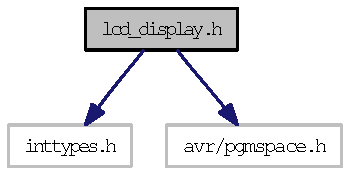
\includegraphics[width=102pt]{lcd__display_8h__incl}
\end{center}
\end{figure}


This graph shows which files directly or indirectly include this file:\nopagebreak
\begin{figure}[H]
\begin{center}
\leavevmode
\includegraphics[width=130pt]{lcd__display_8h__dep__incl}
\end{center}
\end{figure}
\subsection*{Functions}
\begin{CompactItemize}
\item 
\hypertarget{lcd__display_8h_4f1928f1515e21422d5a33af2949f2f7}{
\#define \hyperlink{lcd__display_8h_4f1928f1515e21422d5a33af2949f2f7}{lcd\_\-puts\_\-P}(\_\-\_\-s)~lcd\_\-puts\_\-p(PSTR(\_\-\_\-s))}
\label{lcd__display_8h_4f1928f1515e21422d5a33af2949f2f7}

\begin{CompactList}\small\item\em macros for automatically storing string constant in program memory \item\end{CompactList}\item 
void \hyperlink{lcd__display_8h_9af28b2779326b63ff4356e2b1828984}{lcd\_\-init} (uint8\_\-t dispAttr)
\begin{CompactList}\small\item\em Initialize display and select type of cursor. \item\end{CompactList}\item 
void \hyperlink{lcd__display_8h_f8da853dba4b9d5f2aea4e294444e14d}{lcd\_\-clrscr} (void)
\begin{CompactList}\small\item\em Clear display and set cursor to home position. \item\end{CompactList}\item 
void \hyperlink{lcd__display_8h_3aabf730aa4e0393bb5c959583c00a8e}{lcd\_\-home} (void)
\begin{CompactList}\small\item\em Set cursor to home position. \item\end{CompactList}\item 
void \hyperlink{lcd__display_8h_dbf47a5efdf02367ded1ebf8f9edb5fe}{lcd\_\-gotoxy} (uint8\_\-t x, uint8\_\-t y)
\begin{CompactList}\small\item\em Set cursor to specified position. \item\end{CompactList}\item 
void \hyperlink{lcd__display_8h_fa7e36b95c43d603f510273ad077cbbe}{lcd\_\-putc} (char c)
\begin{CompactList}\small\item\em Display character at current cursor position. \item\end{CompactList}\item 
void \hyperlink{lcd__display_8h_8ffdfcac7638368ff04364c14984266e}{lcd\_\-puts} (const char $\ast$s)
\begin{CompactList}\small\item\em Display string without auto linefeed. \item\end{CompactList}\item 
void \hyperlink{lcd__display_8h_9022a24a56a9b15681f62eb6ba77e5de}{lcd\_\-puts\_\-p} (const char $\ast$progmem\_\-s)
\begin{CompactList}\small\item\em Display string from program memory without auto linefeed. \item\end{CompactList}\item 
void \hyperlink{lcd__display_8h_ea9d14f02df06f948cb5a56776980826}{lcd\_\-command} (uint8\_\-t cmd)
\begin{CompactList}\small\item\em Send LCD controller instruction command. \item\end{CompactList}\item 
void \hyperlink{lcd__display_8h_d0729d2cba627825a089ca1fff12ba29}{lcd\_\-data} (uint8\_\-t data)
\begin{CompactList}\small\item\em Send data byte to LCD controller. \item\end{CompactList}\end{CompactItemize}
\subsection*{Defines}
\begin{Indent}{\bf Definitions for MCU Clock Frequency}\par
{\em Adapt the MCU clock frequency in Hz to your target. }\begin{CompactItemize}
\item 
\#define \hyperlink{lcd__display_8h_3cad0f9b3c40159bd2fbd7f5e60f2fff}{XTAL}~16000000
\end{CompactItemize}
\end{Indent}
\begin{Indent}{\bf Definition for LCD controller type}\par
{\em Use 0 for HD44780 controller, change to 1 for displays with KS0073 controller. }\begin{CompactItemize}
\item 
\#define \hyperlink{lcd__display_8h_63574b03f72a197aeee823aae95dc3b7}{LCD\_\-CONTROLLER\_\-KS0073}~0
\end{CompactItemize}
\end{Indent}
\begin{Indent}{\bf Definitions for Display Size}\par
{\em Change these definitions to adapt setting to your display }\begin{CompactItemize}
\item 
\#define \hyperlink{lcd__display_8h_01212e90283511562039db786f65ba98}{LCD\_\-LINES}~2
\item 
\#define \hyperlink{lcd__display_8h_684bb4392e384b7ae7c660d81dacb930}{LCD\_\-DISP\_\-LENGTH}~24
\item 
\#define \hyperlink{lcd__display_8h_e59a728d9dee9f12c817b29d38746ed9}{LCD\_\-LINE\_\-LENGTH}~0x40
\item 
\#define \hyperlink{lcd__display_8h_bd056d70a1488ea2eb1aef87e248e234}{LCD\_\-START\_\-LINE1}~0x00
\item 
\#define \hyperlink{lcd__display_8h_7b317b21058ef031716ba040ef75430a}{LCD\_\-START\_\-LINE2}~0x40
\item 
\#define \hyperlink{lcd__display_8h_e7cca16353048a062baeb3a52da55249}{LCD\_\-START\_\-LINE3}~0x14
\item 
\#define \hyperlink{lcd__display_8h_b1b73e05bdb5cc12cdff5a1cf6c4f2a2}{LCD\_\-START\_\-LINE4}~0x54
\item 
\#define \hyperlink{lcd__display_8h_db35ff6cb242e48ba0545ea919ffc5d3}{LCD\_\-WRAP\_\-LINES}~0
\item 
\#define \hyperlink{lcd__display_8h_659fcdf979f69bbd14f852f525f25e02}{LCD\_\-IO\_\-MODE}~1
\end{CompactItemize}
\end{Indent}
\begin{Indent}{\bf Definitions for 4-bit IO mode}\par
{\em Change LCD\_\-PORT if you want to use a different port for the LCD pins.

The four LCD data lines and the three control lines RS, RW, E can be on the same port or on different ports. Change LCD\_\-RS\_\-PORT, LCD\_\-RW\_\-PORT, LCD\_\-E\_\-PORT if you want the control lines on different ports.

Normally the four data lines should be mapped to bit 0..3 on one port, but it is possible to connect these data lines in different order or even on different ports by adapting the LCD\_\-DATAx\_\-PORT and LCD\_\-DATAx\_\-PIN definitions. }\begin{CompactItemize}
\item 
\#define \hyperlink{lcd__display_8h_bcf42bd88b3c36193f301ca25b033875}{LCD\_\-PORT}~PORTC
\item 
\#define \hyperlink{lcd__display_8h_fc0acd4774bcd311595732f5367e266b}{LCD\_\-DATA0\_\-PORT}~LCD\_\-PORT
\item 
\#define \hyperlink{lcd__display_8h_345af0248d5739bd8896d4f585618ca2}{LCD\_\-DATA1\_\-PORT}~LCD\_\-PORT
\item 
\#define \hyperlink{lcd__display_8h_4d5c48a3f2b9426c14bbca3150834a20}{LCD\_\-DATA2\_\-PORT}~LCD\_\-PORT
\item 
\#define \hyperlink{lcd__display_8h_ec71b6692f2af7c9de32dbe85fcb51c2}{LCD\_\-DATA3\_\-PORT}~LCD\_\-PORT
\item 
\#define \hyperlink{lcd__display_8h_fe54d7d886b5c56bed0cf971febbb773}{LCD\_\-DATA0\_\-PIN}~2
\item 
\#define \hyperlink{lcd__display_8h_97fb520e7b83bb047ac5c9247de57049}{LCD\_\-DATA1\_\-PIN}~3
\item 
\#define \hyperlink{lcd__display_8h_7f3d53627337f6535cc8daa35876510a}{LCD\_\-DATA2\_\-PIN}~4
\item 
\#define \hyperlink{lcd__display_8h_54032ce0050853e181f879b69fec4370}{LCD\_\-DATA3\_\-PIN}~5
\item 
\#define \hyperlink{lcd__display_8h_c5be2a22727fd9ca349e1c9bcbfbcd47}{LCD\_\-RS\_\-PORT}~LCD\_\-PORT
\item 
\#define \hyperlink{lcd__display_8h_e5c0a0a5750f3aaea06083e3a4a31f5d}{LCD\_\-RS\_\-PIN}~7
\item 
\#define \hyperlink{lcd__display_8h_e8772bdf31db863b81805c837bdc2da2}{LCD\_\-RW\_\-PORT}~PORTD
\item 
\#define \hyperlink{lcd__display_8h_3ac938dd5fc02a9a232df6605b5f6aa8}{LCD\_\-RW\_\-PIN}~3
\item 
\#define \hyperlink{lcd__display_8h_f97f97ff3832d1289bbcb471090ea297}{LCD\_\-E\_\-PORT}~LCD\_\-PORT
\item 
\#define \hyperlink{lcd__display_8h_e644d776392a8d47899d9910c2b8feb6}{LCD\_\-E\_\-PIN}~6
\end{CompactItemize}
\end{Indent}
\begin{Indent}{\bf Definitions for LCD command instructions}\par
{\em The constants define the various LCD controller instructions which can be passed to the function \hyperlink{lcd__display_8c_ea9d14f02df06f948cb5a56776980826}{lcd\_\-command()}, see HD44780 data sheet for a complete description. }\begin{CompactItemize}
\item 
\hypertarget{lcd__display_8h_459688213267d13ccfbeb2c9004988cb}{
\#define \textbf{LCD\_\-CLR}~0}
\label{lcd__display_8h_459688213267d13ccfbeb2c9004988cb}

\item 
\hypertarget{lcd__display_8h_e0e309ccad89222eb3457f2da9f2bb8d}{
\#define \textbf{LCD\_\-HOME}~1}
\label{lcd__display_8h_e0e309ccad89222eb3457f2da9f2bb8d}

\item 
\hypertarget{lcd__display_8h_e5d757ddb6d94de8c82191b60b40e442}{
\#define \textbf{LCD\_\-ENTRY\_\-MODE}~2}
\label{lcd__display_8h_e5d757ddb6d94de8c82191b60b40e442}

\item 
\hypertarget{lcd__display_8h_da766266a0be0d0040fbf86e23b58aa6}{
\#define \textbf{LCD\_\-ENTRY\_\-INC}~1}
\label{lcd__display_8h_da766266a0be0d0040fbf86e23b58aa6}

\item 
\hypertarget{lcd__display_8h_14d0c7fda147e0dc8cdaa4a2629b3532}{
\#define \textbf{LCD\_\-ENTRY\_\-SHIFT}~0}
\label{lcd__display_8h_14d0c7fda147e0dc8cdaa4a2629b3532}

\item 
\hypertarget{lcd__display_8h_47a809dfec086fdeca93dedc4fb83b44}{
\#define \textbf{LCD\_\-ON}~3}
\label{lcd__display_8h_47a809dfec086fdeca93dedc4fb83b44}

\item 
\hypertarget{lcd__display_8h_e84f634b0a1661c4d5bbaafd9397732a}{
\#define \textbf{LCD\_\-ON\_\-DISPLAY}~2}
\label{lcd__display_8h_e84f634b0a1661c4d5bbaafd9397732a}

\item 
\hypertarget{lcd__display_8h_47638b5ebbaec9600a0ebf9a55caf802}{
\#define \textbf{LCD\_\-ON\_\-CURSOR}~1}
\label{lcd__display_8h_47638b5ebbaec9600a0ebf9a55caf802}

\item 
\hypertarget{lcd__display_8h_5d76592a978537acee615098ce4d80f5}{
\#define \textbf{LCD\_\-ON\_\-BLINK}~0}
\label{lcd__display_8h_5d76592a978537acee615098ce4d80f5}

\item 
\hypertarget{lcd__display_8h_3f4f758b80fcfa6c9e4db58e2515c78a}{
\#define \textbf{LCD\_\-MOVE}~4}
\label{lcd__display_8h_3f4f758b80fcfa6c9e4db58e2515c78a}

\item 
\hypertarget{lcd__display_8h_addc2afa9a02bfa748950f2c1e6a204d}{
\#define \textbf{LCD\_\-MOVE\_\-DISP}~3}
\label{lcd__display_8h_addc2afa9a02bfa748950f2c1e6a204d}

\item 
\hypertarget{lcd__display_8h_97cdb19acf109ad52ab4994d2ad02cee}{
\#define \textbf{LCD\_\-MOVE\_\-RIGHT}~2}
\label{lcd__display_8h_97cdb19acf109ad52ab4994d2ad02cee}

\item 
\hypertarget{lcd__display_8h_50de1697f1da8ab075a6b4d7aeace64e}{
\#define \textbf{LCD\_\-FUNCTION}~5}
\label{lcd__display_8h_50de1697f1da8ab075a6b4d7aeace64e}

\item 
\hypertarget{lcd__display_8h_91d15d8e3008f6cb141406a8b5d0d3c0}{
\#define \textbf{LCD\_\-FUNCTION\_\-8BIT}~4}
\label{lcd__display_8h_91d15d8e3008f6cb141406a8b5d0d3c0}

\item 
\hypertarget{lcd__display_8h_6c24806bed18d565917165caa3475463}{
\#define \textbf{LCD\_\-FUNCTION\_\-2LINES}~3}
\label{lcd__display_8h_6c24806bed18d565917165caa3475463}

\item 
\hypertarget{lcd__display_8h_48de81358277fe4f2810c2b82f90397e}{
\#define \textbf{LCD\_\-FUNCTION\_\-10DOTS}~2}
\label{lcd__display_8h_48de81358277fe4f2810c2b82f90397e}

\item 
\hypertarget{lcd__display_8h_3b38de74c362be1781fef1136aa9684c}{
\#define \textbf{LCD\_\-CGRAM}~6}
\label{lcd__display_8h_3b38de74c362be1781fef1136aa9684c}

\item 
\hypertarget{lcd__display_8h_e54acf3ccc45b7d6be334a03627740c6}{
\#define \textbf{LCD\_\-DDRAM}~7}
\label{lcd__display_8h_e54acf3ccc45b7d6be334a03627740c6}

\item 
\hypertarget{lcd__display_8h_c8dd1658e235f174d1cabae5c438943d}{
\#define \textbf{LCD\_\-BUSY}~7}
\label{lcd__display_8h_c8dd1658e235f174d1cabae5c438943d}

\item 
\hypertarget{lcd__display_8h_ad56f8e07634e85663f56888ae97089c}{
\#define \textbf{LCD\_\-ENTRY\_\-DEC}~0x04}
\label{lcd__display_8h_ad56f8e07634e85663f56888ae97089c}

\item 
\hypertarget{lcd__display_8h_1c62932f252c6262cbef728add9696e4}{
\#define \textbf{LCD\_\-ENTRY\_\-DEC\_\-SHIFT}~0x05}
\label{lcd__display_8h_1c62932f252c6262cbef728add9696e4}

\item 
\hypertarget{lcd__display_8h_d27ddc4b8d03594662c8757f946dde28}{
\#define \textbf{LCD\_\-ENTRY\_\-INC\_\-}~0x06}
\label{lcd__display_8h_d27ddc4b8d03594662c8757f946dde28}

\item 
\hypertarget{lcd__display_8h_fabd0215cc6ae5539dc638dbec44a506}{
\#define \textbf{LCD\_\-ENTRY\_\-INC\_\-SHIFT}~0x07}
\label{lcd__display_8h_fabd0215cc6ae5539dc638dbec44a506}

\item 
\hypertarget{lcd__display_8h_a2966175115943883f51e9c90478540c}{
\#define \textbf{LCD\_\-DISP\_\-OFF}~0x08}
\label{lcd__display_8h_a2966175115943883f51e9c90478540c}

\item 
\hypertarget{lcd__display_8h_5163a96b133868975c0738e180b30cb8}{
\#define \textbf{LCD\_\-DISP\_\-ON}~0x0C}
\label{lcd__display_8h_5163a96b133868975c0738e180b30cb8}

\item 
\hypertarget{lcd__display_8h_470cef85de53e37356b22c66a357a764}{
\#define \textbf{LCD\_\-DISP\_\-ON\_\-BLINK}~0x0D}
\label{lcd__display_8h_470cef85de53e37356b22c66a357a764}

\item 
\hypertarget{lcd__display_8h_f56b6d6bdb6fa48b26106dee5f74ae1f}{
\#define \textbf{LCD\_\-DISP\_\-ON\_\-CURSOR}~0x0E}
\label{lcd__display_8h_f56b6d6bdb6fa48b26106dee5f74ae1f}

\item 
\hypertarget{lcd__display_8h_c1984ed0db15c6991d34c184fdca5dc6}{
\#define \textbf{LCD\_\-DISP\_\-ON\_\-CURSOR\_\-BLINK}~0x0F}
\label{lcd__display_8h_c1984ed0db15c6991d34c184fdca5dc6}

\item 
\hypertarget{lcd__display_8h_c2f0ddce1daaa1bf1a016270a89a264b}{
\#define \textbf{LCD\_\-MOVE\_\-CURSOR\_\-LEFT}~0x10}
\label{lcd__display_8h_c2f0ddce1daaa1bf1a016270a89a264b}

\item 
\hypertarget{lcd__display_8h_0ad58e39e053e97d34527fcbe936899b}{
\#define \textbf{LCD\_\-MOVE\_\-CURSOR\_\-RIGHT}~0x14}
\label{lcd__display_8h_0ad58e39e053e97d34527fcbe936899b}

\item 
\hypertarget{lcd__display_8h_b3c34ff1eee238bbe9c677215219fb8e}{
\#define \textbf{LCD\_\-MOVE\_\-DISP\_\-LEFT}~0x18}
\label{lcd__display_8h_b3c34ff1eee238bbe9c677215219fb8e}

\item 
\hypertarget{lcd__display_8h_9a90bb926f5ba59378af81fe8e246ffb}{
\#define \textbf{LCD\_\-MOVE\_\-DISP\_\-RIGHT}~0x1C}
\label{lcd__display_8h_9a90bb926f5ba59378af81fe8e246ffb}

\item 
\hypertarget{lcd__display_8h_ff4e5baa36a0322eb97557dcb18cd96e}{
\#define \textbf{LCD\_\-FUNCTION\_\-4BIT\_\-1LINE}~0x20}
\label{lcd__display_8h_ff4e5baa36a0322eb97557dcb18cd96e}

\item 
\hypertarget{lcd__display_8h_b35032ab368a8bc90798e0c547fb24c2}{
\#define \textbf{LCD\_\-FUNCTION\_\-4BIT\_\-2LINES}~0x28}
\label{lcd__display_8h_b35032ab368a8bc90798e0c547fb24c2}

\item 
\hypertarget{lcd__display_8h_a8aeee098cb4c84ec420e00d054abcce}{
\#define \textbf{LCD\_\-FUNCTION\_\-8BIT\_\-1LINE}~0x30}
\label{lcd__display_8h_a8aeee098cb4c84ec420e00d054abcce}

\item 
\hypertarget{lcd__display_8h_160a214f47869f8f98ad5add3a7568db}{
\#define \textbf{LCD\_\-FUNCTION\_\-8BIT\_\-2LINES}~0x38}
\label{lcd__display_8h_160a214f47869f8f98ad5add3a7568db}

\item 
\hypertarget{lcd__display_8h_1849e2087d3034a3fffa67444beed109}{
\#define \textbf{LCD\_\-MODE\_\-DEFAULT}~((1$<$$<$LCD\_\-ENTRY\_\-MODE) $|$ (1$<$$<$LCD\_\-ENTRY\_\-INC) )}
\label{lcd__display_8h_1849e2087d3034a3fffa67444beed109}

\end{CompactItemize}
\end{Indent}


\subsection{Detailed Description}
Basic routines for interfacing a HD44780U-based text LCD display. 

\hypertarget{index_intro}{}\subsection{License}\label{index_intro}


\begin{Code}\begin{verbatim} Originally based on Volker Oth's LCD library,
 changed lcd_init(), added additional constants for lcd_command(), 
 added 4-bit I/O mode, improved and optimized code.
       
 Library can be operated in memory mapped mode (LCD_IO_MODE=0) or in 
 4-bit IO port mode (LCD_IO_MODE=1). 8-bit IO port mode not supported.

 Memory mapped mode compatible with Kanda STK200, but supports also 
 generation of R/W signal through A8 address line.
\end{verbatim}
\end{Code}



\begin{Desc}
\item[Author:]Peter Fleury \href{mailto:pfleury@gmx.ch}{\tt pfleury@gmx.ch} \href{http://jump.to/fleury}{\tt http://jump.to/fleury}\end{Desc}
\begin{Desc}
\item[See also:]The chapter \href{http://homepage.sunrise.ch/mysunrise/peterfleury/avr-lcd44780.html}{\tt Interfacing a HD44780 Based LCD to an AVR} on my home page.\end{Desc}
Further documentation can be found in \hyperlink{lcd__display_8c}{lcd\_\-display.c} 

Definition in file \hyperlink{lcd__display_8h-source}{lcd\_\-display.h}.

\subsection{Define Documentation}
\hypertarget{lcd__display_8h_63574b03f72a197aeee823aae95dc3b7}{
\index{lcd\_\-display.h@{lcd\_\-display.h}!LCD\_\-CONTROLLER\_\-KS0073@{LCD\_\-CONTROLLER\_\-KS0073}}
\index{LCD\_\-CONTROLLER\_\-KS0073@{LCD\_\-CONTROLLER\_\-KS0073}!lcd_display.h@{lcd\_\-display.h}}
\subsubsection{\setlength{\rightskip}{0pt plus 5cm}\#define LCD\_\-CONTROLLER\_\-KS0073~0}}
\label{lcd__display_8h_63574b03f72a197aeee823aae95dc3b7}


Use 0 for HD44780 controller, 1 for KS0073 controller 

Definition at line 55 of file lcd\_\-display.h.\hypertarget{lcd__display_8h_fe54d7d886b5c56bed0cf971febbb773}{
\index{lcd\_\-display.h@{lcd\_\-display.h}!LCD\_\-DATA0\_\-PIN@{LCD\_\-DATA0\_\-PIN}}
\index{LCD\_\-DATA0\_\-PIN@{LCD\_\-DATA0\_\-PIN}!lcd_display.h@{lcd\_\-display.h}}
\subsubsection{\setlength{\rightskip}{0pt plus 5cm}\#define LCD\_\-DATA0\_\-PIN~2}}
\label{lcd__display_8h_fe54d7d886b5c56bed0cf971febbb773}


pin for 4bit data bit 0 

Definition at line 92 of file lcd\_\-display.h.

Referenced by lcd\_\-init().\hypertarget{lcd__display_8h_fc0acd4774bcd311595732f5367e266b}{
\index{lcd\_\-display.h@{lcd\_\-display.h}!LCD\_\-DATA0\_\-PORT@{LCD\_\-DATA0\_\-PORT}}
\index{LCD\_\-DATA0\_\-PORT@{LCD\_\-DATA0\_\-PORT}!lcd_display.h@{lcd\_\-display.h}}
\subsubsection{\setlength{\rightskip}{0pt plus 5cm}\#define LCD\_\-DATA0\_\-PORT~LCD\_\-PORT}}
\label{lcd__display_8h_fc0acd4774bcd311595732f5367e266b}


port for 4bit data bit 0 

Definition at line 88 of file lcd\_\-display.h.

Referenced by lcd\_\-init().\hypertarget{lcd__display_8h_97fb520e7b83bb047ac5c9247de57049}{
\index{lcd\_\-display.h@{lcd\_\-display.h}!LCD\_\-DATA1\_\-PIN@{LCD\_\-DATA1\_\-PIN}}
\index{LCD\_\-DATA1\_\-PIN@{LCD\_\-DATA1\_\-PIN}!lcd_display.h@{lcd\_\-display.h}}
\subsubsection{\setlength{\rightskip}{0pt plus 5cm}\#define LCD\_\-DATA1\_\-PIN~3}}
\label{lcd__display_8h_97fb520e7b83bb047ac5c9247de57049}


pin for 4bit data bit 1 

Definition at line 93 of file lcd\_\-display.h.

Referenced by lcd\_\-init().\hypertarget{lcd__display_8h_345af0248d5739bd8896d4f585618ca2}{
\index{lcd\_\-display.h@{lcd\_\-display.h}!LCD\_\-DATA1\_\-PORT@{LCD\_\-DATA1\_\-PORT}}
\index{LCD\_\-DATA1\_\-PORT@{LCD\_\-DATA1\_\-PORT}!lcd_display.h@{lcd\_\-display.h}}
\subsubsection{\setlength{\rightskip}{0pt plus 5cm}\#define LCD\_\-DATA1\_\-PORT~LCD\_\-PORT}}
\label{lcd__display_8h_345af0248d5739bd8896d4f585618ca2}


port for 4bit data bit 1 

Definition at line 89 of file lcd\_\-display.h.

Referenced by lcd\_\-init().\hypertarget{lcd__display_8h_7f3d53627337f6535cc8daa35876510a}{
\index{lcd\_\-display.h@{lcd\_\-display.h}!LCD\_\-DATA2\_\-PIN@{LCD\_\-DATA2\_\-PIN}}
\index{LCD\_\-DATA2\_\-PIN@{LCD\_\-DATA2\_\-PIN}!lcd_display.h@{lcd\_\-display.h}}
\subsubsection{\setlength{\rightskip}{0pt plus 5cm}\#define LCD\_\-DATA2\_\-PIN~4}}
\label{lcd__display_8h_7f3d53627337f6535cc8daa35876510a}


pin for 4bit data bit 2 

Definition at line 94 of file lcd\_\-display.h.

Referenced by lcd\_\-init().\hypertarget{lcd__display_8h_4d5c48a3f2b9426c14bbca3150834a20}{
\index{lcd\_\-display.h@{lcd\_\-display.h}!LCD\_\-DATA2\_\-PORT@{LCD\_\-DATA2\_\-PORT}}
\index{LCD\_\-DATA2\_\-PORT@{LCD\_\-DATA2\_\-PORT}!lcd_display.h@{lcd\_\-display.h}}
\subsubsection{\setlength{\rightskip}{0pt plus 5cm}\#define LCD\_\-DATA2\_\-PORT~LCD\_\-PORT}}
\label{lcd__display_8h_4d5c48a3f2b9426c14bbca3150834a20}


port for 4bit data bit 2 

Definition at line 90 of file lcd\_\-display.h.

Referenced by lcd\_\-init().\hypertarget{lcd__display_8h_54032ce0050853e181f879b69fec4370}{
\index{lcd\_\-display.h@{lcd\_\-display.h}!LCD\_\-DATA3\_\-PIN@{LCD\_\-DATA3\_\-PIN}}
\index{LCD\_\-DATA3\_\-PIN@{LCD\_\-DATA3\_\-PIN}!lcd_display.h@{lcd\_\-display.h}}
\subsubsection{\setlength{\rightskip}{0pt plus 5cm}\#define LCD\_\-DATA3\_\-PIN~5}}
\label{lcd__display_8h_54032ce0050853e181f879b69fec4370}


pin for 4bit data bit 3 

Definition at line 95 of file lcd\_\-display.h.

Referenced by lcd\_\-init().\hypertarget{lcd__display_8h_ec71b6692f2af7c9de32dbe85fcb51c2}{
\index{lcd\_\-display.h@{lcd\_\-display.h}!LCD\_\-DATA3\_\-PORT@{LCD\_\-DATA3\_\-PORT}}
\index{LCD\_\-DATA3\_\-PORT@{LCD\_\-DATA3\_\-PORT}!lcd_display.h@{lcd\_\-display.h}}
\subsubsection{\setlength{\rightskip}{0pt plus 5cm}\#define LCD\_\-DATA3\_\-PORT~LCD\_\-PORT}}
\label{lcd__display_8h_ec71b6692f2af7c9de32dbe85fcb51c2}


port for 4bit data bit 3 

Definition at line 91 of file lcd\_\-display.h.

Referenced by lcd\_\-init().\hypertarget{lcd__display_8h_684bb4392e384b7ae7c660d81dacb930}{
\index{lcd\_\-display.h@{lcd\_\-display.h}!LCD\_\-DISP\_\-LENGTH@{LCD\_\-DISP\_\-LENGTH}}
\index{LCD\_\-DISP\_\-LENGTH@{LCD\_\-DISP\_\-LENGTH}!lcd_display.h@{lcd\_\-display.h}}
\subsubsection{\setlength{\rightskip}{0pt plus 5cm}\#define LCD\_\-DISP\_\-LENGTH~24}}
\label{lcd__display_8h_684bb4392e384b7ae7c660d81dacb930}


visibles characters per line of the display 

Definition at line 62 of file lcd\_\-display.h.

Referenced by lcd\_\-putc().\hypertarget{lcd__display_8h_e644d776392a8d47899d9910c2b8feb6}{
\index{lcd\_\-display.h@{lcd\_\-display.h}!LCD\_\-E\_\-PIN@{LCD\_\-E\_\-PIN}}
\index{LCD\_\-E\_\-PIN@{LCD\_\-E\_\-PIN}!lcd_display.h@{lcd\_\-display.h}}
\subsubsection{\setlength{\rightskip}{0pt plus 5cm}\#define LCD\_\-E\_\-PIN~6}}
\label{lcd__display_8h_e644d776392a8d47899d9910c2b8feb6}


pin for Enable line 

Definition at line 101 of file lcd\_\-display.h.

Referenced by lcd\_\-init().\hypertarget{lcd__display_8h_f97f97ff3832d1289bbcb471090ea297}{
\index{lcd\_\-display.h@{lcd\_\-display.h}!LCD\_\-E\_\-PORT@{LCD\_\-E\_\-PORT}}
\index{LCD\_\-E\_\-PORT@{LCD\_\-E\_\-PORT}!lcd_display.h@{lcd\_\-display.h}}
\subsubsection{\setlength{\rightskip}{0pt plus 5cm}\#define LCD\_\-E\_\-PORT~LCD\_\-PORT}}
\label{lcd__display_8h_f97f97ff3832d1289bbcb471090ea297}


port for Enable line 

Definition at line 100 of file lcd\_\-display.h.

Referenced by lcd\_\-init().\hypertarget{lcd__display_8h_659fcdf979f69bbd14f852f525f25e02}{
\index{lcd\_\-display.h@{lcd\_\-display.h}!LCD\_\-IO\_\-MODE@{LCD\_\-IO\_\-MODE}}
\index{LCD\_\-IO\_\-MODE@{LCD\_\-IO\_\-MODE}!lcd_display.h@{lcd\_\-display.h}}
\subsubsection{\setlength{\rightskip}{0pt plus 5cm}\#define LCD\_\-IO\_\-MODE~1}}
\label{lcd__display_8h_659fcdf979f69bbd14f852f525f25e02}


0: memory mapped mode, 1: IO port mode 

Definition at line 71 of file lcd\_\-display.h.\hypertarget{lcd__display_8h_e59a728d9dee9f12c817b29d38746ed9}{
\index{lcd\_\-display.h@{lcd\_\-display.h}!LCD\_\-LINE\_\-LENGTH@{LCD\_\-LINE\_\-LENGTH}}
\index{LCD\_\-LINE\_\-LENGTH@{LCD\_\-LINE\_\-LENGTH}!lcd_display.h@{lcd\_\-display.h}}
\subsubsection{\setlength{\rightskip}{0pt plus 5cm}\#define LCD\_\-LINE\_\-LENGTH~0x40}}
\label{lcd__display_8h_e59a728d9dee9f12c817b29d38746ed9}


internal line length of the display 

Definition at line 63 of file lcd\_\-display.h.\hypertarget{lcd__display_8h_01212e90283511562039db786f65ba98}{
\index{lcd\_\-display.h@{lcd\_\-display.h}!LCD\_\-LINES@{LCD\_\-LINES}}
\index{LCD\_\-LINES@{LCD\_\-LINES}!lcd_display.h@{lcd\_\-display.h}}
\subsubsection{\setlength{\rightskip}{0pt plus 5cm}\#define LCD\_\-LINES~2}}
\label{lcd__display_8h_01212e90283511562039db786f65ba98}


number of visible lines of the display 

Definition at line 61 of file lcd\_\-display.h.\hypertarget{lcd__display_8h_bcf42bd88b3c36193f301ca25b033875}{
\index{lcd\_\-display.h@{lcd\_\-display.h}!LCD\_\-PORT@{LCD\_\-PORT}}
\index{LCD\_\-PORT@{LCD\_\-PORT}!lcd_display.h@{lcd\_\-display.h}}
\subsubsection{\setlength{\rightskip}{0pt plus 5cm}\#define LCD\_\-PORT~PORTC}}
\label{lcd__display_8h_bcf42bd88b3c36193f301ca25b033875}


port for the LCD lines 

Definition at line 87 of file lcd\_\-display.h.\hypertarget{lcd__display_8h_e5c0a0a5750f3aaea06083e3a4a31f5d}{
\index{lcd\_\-display.h@{lcd\_\-display.h}!LCD\_\-RS\_\-PIN@{LCD\_\-RS\_\-PIN}}
\index{LCD\_\-RS\_\-PIN@{LCD\_\-RS\_\-PIN}!lcd_display.h@{lcd\_\-display.h}}
\subsubsection{\setlength{\rightskip}{0pt plus 5cm}\#define LCD\_\-RS\_\-PIN~7}}
\label{lcd__display_8h_e5c0a0a5750f3aaea06083e3a4a31f5d}


pin for RS line 

Definition at line 97 of file lcd\_\-display.h.

Referenced by lcd\_\-init().\hypertarget{lcd__display_8h_c5be2a22727fd9ca349e1c9bcbfbcd47}{
\index{lcd\_\-display.h@{lcd\_\-display.h}!LCD\_\-RS\_\-PORT@{LCD\_\-RS\_\-PORT}}
\index{LCD\_\-RS\_\-PORT@{LCD\_\-RS\_\-PORT}!lcd_display.h@{lcd\_\-display.h}}
\subsubsection{\setlength{\rightskip}{0pt plus 5cm}\#define LCD\_\-RS\_\-PORT~LCD\_\-PORT}}
\label{lcd__display_8h_c5be2a22727fd9ca349e1c9bcbfbcd47}


port for RS line 

Definition at line 96 of file lcd\_\-display.h.

Referenced by lcd\_\-init().\hypertarget{lcd__display_8h_3ac938dd5fc02a9a232df6605b5f6aa8}{
\index{lcd\_\-display.h@{lcd\_\-display.h}!LCD\_\-RW\_\-PIN@{LCD\_\-RW\_\-PIN}}
\index{LCD\_\-RW\_\-PIN@{LCD\_\-RW\_\-PIN}!lcd_display.h@{lcd\_\-display.h}}
\subsubsection{\setlength{\rightskip}{0pt plus 5cm}\#define LCD\_\-RW\_\-PIN~3}}
\label{lcd__display_8h_3ac938dd5fc02a9a232df6605b5f6aa8}


pin for RW line 

Definition at line 99 of file lcd\_\-display.h.

Referenced by lcd\_\-init().\hypertarget{lcd__display_8h_e8772bdf31db863b81805c837bdc2da2}{
\index{lcd\_\-display.h@{lcd\_\-display.h}!LCD\_\-RW\_\-PORT@{LCD\_\-RW\_\-PORT}}
\index{LCD\_\-RW\_\-PORT@{LCD\_\-RW\_\-PORT}!lcd_display.h@{lcd\_\-display.h}}
\subsubsection{\setlength{\rightskip}{0pt plus 5cm}\#define LCD\_\-RW\_\-PORT~PORTD}}
\label{lcd__display_8h_e8772bdf31db863b81805c837bdc2da2}


port for RW line 

Definition at line 98 of file lcd\_\-display.h.

Referenced by lcd\_\-init().\hypertarget{lcd__display_8h_bd056d70a1488ea2eb1aef87e248e234}{
\index{lcd\_\-display.h@{lcd\_\-display.h}!LCD\_\-START\_\-LINE1@{LCD\_\-START\_\-LINE1}}
\index{LCD\_\-START\_\-LINE1@{LCD\_\-START\_\-LINE1}!lcd_display.h@{lcd\_\-display.h}}
\subsubsection{\setlength{\rightskip}{0pt plus 5cm}\#define LCD\_\-START\_\-LINE1~0x00}}
\label{lcd__display_8h_bd056d70a1488ea2eb1aef87e248e234}


DDRAM address of first char of line 1 

Definition at line 64 of file lcd\_\-display.h.

Referenced by lcd\_\-gotoxy(), and lcd\_\-putc().\hypertarget{lcd__display_8h_7b317b21058ef031716ba040ef75430a}{
\index{lcd\_\-display.h@{lcd\_\-display.h}!LCD\_\-START\_\-LINE2@{LCD\_\-START\_\-LINE2}}
\index{LCD\_\-START\_\-LINE2@{LCD\_\-START\_\-LINE2}!lcd_display.h@{lcd\_\-display.h}}
\subsubsection{\setlength{\rightskip}{0pt plus 5cm}\#define LCD\_\-START\_\-LINE2~0x40}}
\label{lcd__display_8h_7b317b21058ef031716ba040ef75430a}


DDRAM address of first char of line 2 

Definition at line 65 of file lcd\_\-display.h.

Referenced by lcd\_\-gotoxy(), and lcd\_\-putc().\hypertarget{lcd__display_8h_e7cca16353048a062baeb3a52da55249}{
\index{lcd\_\-display.h@{lcd\_\-display.h}!LCD\_\-START\_\-LINE3@{LCD\_\-START\_\-LINE3}}
\index{LCD\_\-START\_\-LINE3@{LCD\_\-START\_\-LINE3}!lcd_display.h@{lcd\_\-display.h}}
\subsubsection{\setlength{\rightskip}{0pt plus 5cm}\#define LCD\_\-START\_\-LINE3~0x14}}
\label{lcd__display_8h_e7cca16353048a062baeb3a52da55249}


DDRAM address of first char of line 3 

Definition at line 66 of file lcd\_\-display.h.

Referenced by lcd\_\-gotoxy(), and lcd\_\-putc().\hypertarget{lcd__display_8h_b1b73e05bdb5cc12cdff5a1cf6c4f2a2}{
\index{lcd\_\-display.h@{lcd\_\-display.h}!LCD\_\-START\_\-LINE4@{LCD\_\-START\_\-LINE4}}
\index{LCD\_\-START\_\-LINE4@{LCD\_\-START\_\-LINE4}!lcd_display.h@{lcd\_\-display.h}}
\subsubsection{\setlength{\rightskip}{0pt plus 5cm}\#define LCD\_\-START\_\-LINE4~0x54}}
\label{lcd__display_8h_b1b73e05bdb5cc12cdff5a1cf6c4f2a2}


DDRAM address of first char of line 4 

Definition at line 67 of file lcd\_\-display.h.

Referenced by lcd\_\-gotoxy(), and lcd\_\-putc().\hypertarget{lcd__display_8h_db35ff6cb242e48ba0545ea919ffc5d3}{
\index{lcd\_\-display.h@{lcd\_\-display.h}!LCD\_\-WRAP\_\-LINES@{LCD\_\-WRAP\_\-LINES}}
\index{LCD\_\-WRAP\_\-LINES@{LCD\_\-WRAP\_\-LINES}!lcd_display.h@{lcd\_\-display.h}}
\subsubsection{\setlength{\rightskip}{0pt plus 5cm}\#define LCD\_\-WRAP\_\-LINES~0}}
\label{lcd__display_8h_db35ff6cb242e48ba0545ea919ffc5d3}


0: no wrap, 1: wrap at end of visibile line 

Definition at line 68 of file lcd\_\-display.h.\hypertarget{lcd__display_8h_3cad0f9b3c40159bd2fbd7f5e60f2fff}{
\index{lcd\_\-display.h@{lcd\_\-display.h}!XTAL@{XTAL}}
\index{XTAL@{XTAL}!lcd_display.h@{lcd\_\-display.h}}
\subsubsection{\setlength{\rightskip}{0pt plus 5cm}\#define XTAL~16000000}}
\label{lcd__display_8h_3cad0f9b3c40159bd2fbd7f5e60f2fff}


clock frequency in Hz, used to calculate delay timer 

Definition at line 48 of file lcd\_\-display.h.

\subsection{Function Documentation}
\hypertarget{lcd__display_8h_f8da853dba4b9d5f2aea4e294444e14d}{
\index{lcd\_\-display.h@{lcd\_\-display.h}!lcd\_\-clrscr@{lcd\_\-clrscr}}
\index{lcd\_\-clrscr@{lcd\_\-clrscr}!lcd_display.h@{lcd\_\-display.h}}
\subsubsection{\setlength{\rightskip}{0pt plus 5cm}void lcd\_\-clrscr (void)}}
\label{lcd__display_8h_f8da853dba4b9d5f2aea4e294444e14d}


Clear display and set cursor to home position. 

\begin{Desc}
\item[Parameters:]
\begin{description}
\item[{\em void}]\end{description}
\end{Desc}
\begin{Desc}
\item[Returns:]none \end{Desc}


Definition at line 434 of file lcd\_\-display.c.

References lcd\_\-command().

Referenced by init\_\-all(), lcd\_\-init(), and main().\hypertarget{lcd__display_8h_ea9d14f02df06f948cb5a56776980826}{
\index{lcd\_\-display.h@{lcd\_\-display.h}!lcd\_\-command@{lcd\_\-command}}
\index{lcd\_\-command@{lcd\_\-command}!lcd_display.h@{lcd\_\-display.h}}
\subsubsection{\setlength{\rightskip}{0pt plus 5cm}void lcd\_\-command (uint8\_\-t {\em cmd})}}
\label{lcd__display_8h_ea9d14f02df06f948cb5a56776980826}


Send LCD controller instruction command. 

\begin{Desc}
\item[Parameters:]
\begin{description}
\item[{\em cmd}]instruction to send to LCD controller, see HD44780 data sheet \end{description}
\end{Desc}
\begin{Desc}
\item[Returns:]none \end{Desc}


Definition at line 372 of file lcd\_\-display.c.

Referenced by lcd\_\-clrscr(), lcd\_\-gotoxy(), lcd\_\-home(), and lcd\_\-init().\hypertarget{lcd__display_8h_d0729d2cba627825a089ca1fff12ba29}{
\index{lcd\_\-display.h@{lcd\_\-display.h}!lcd\_\-data@{lcd\_\-data}}
\index{lcd\_\-data@{lcd\_\-data}!lcd_display.h@{lcd\_\-display.h}}
\subsubsection{\setlength{\rightskip}{0pt plus 5cm}void lcd\_\-data (uint8\_\-t {\em data})}}
\label{lcd__display_8h_d0729d2cba627825a089ca1fff12ba29}


Send data byte to LCD controller. 

Similar to \hyperlink{lcd__display_8c_fa7e36b95c43d603f510273ad077cbbe}{lcd\_\-putc()}, but without interpreting LF \begin{Desc}
\item[Parameters:]
\begin{description}
\item[{\em data}]byte to send to LCD controller, see HD44780 data sheet \end{description}
\end{Desc}
\begin{Desc}
\item[Returns:]none \end{Desc}


Definition at line 384 of file lcd\_\-display.c.\hypertarget{lcd__display_8h_dbf47a5efdf02367ded1ebf8f9edb5fe}{
\index{lcd\_\-display.h@{lcd\_\-display.h}!lcd\_\-gotoxy@{lcd\_\-gotoxy}}
\index{lcd\_\-gotoxy@{lcd\_\-gotoxy}!lcd_display.h@{lcd\_\-display.h}}
\subsubsection{\setlength{\rightskip}{0pt plus 5cm}void lcd\_\-gotoxy (uint8\_\-t {\em x}, \/  uint8\_\-t {\em y})}}
\label{lcd__display_8h_dbf47a5efdf02367ded1ebf8f9edb5fe}


Set cursor to specified position. 

\begin{Desc}
\item[Parameters:]
\begin{description}
\item[{\em x}]horizontal position\par
 (0: left most position) \item[{\em y}]vertical position\par
 (0: first line) \end{description}
\end{Desc}
\begin{Desc}
\item[Returns:]none \end{Desc}


Definition at line 398 of file lcd\_\-display.c.

References lcd\_\-command(), LCD\_\-START\_\-LINE1, LCD\_\-START\_\-LINE2, LCD\_\-START\_\-LINE3, and LCD\_\-START\_\-LINE4.

Referenced by main().\hypertarget{lcd__display_8h_3aabf730aa4e0393bb5c959583c00a8e}{
\index{lcd\_\-display.h@{lcd\_\-display.h}!lcd\_\-home@{lcd\_\-home}}
\index{lcd\_\-home@{lcd\_\-home}!lcd_display.h@{lcd\_\-display.h}}
\subsubsection{\setlength{\rightskip}{0pt plus 5cm}void lcd\_\-home (void)}}
\label{lcd__display_8h_3aabf730aa4e0393bb5c959583c00a8e}


Set cursor to home position. 

\begin{Desc}
\item[Parameters:]
\begin{description}
\item[{\em void}]\end{description}
\end{Desc}
\begin{Desc}
\item[Returns:]none \end{Desc}


Definition at line 443 of file lcd\_\-display.c.

References lcd\_\-command().\hypertarget{lcd__display_8h_9af28b2779326b63ff4356e2b1828984}{
\index{lcd\_\-display.h@{lcd\_\-display.h}!lcd\_\-init@{lcd\_\-init}}
\index{lcd\_\-init@{lcd\_\-init}!lcd_display.h@{lcd\_\-display.h}}
\subsubsection{\setlength{\rightskip}{0pt plus 5cm}void lcd\_\-init (uint8\_\-t {\em dispAttr})}}
\label{lcd__display_8h_9af28b2779326b63ff4356e2b1828984}


Initialize display and select type of cursor. 

\begin{Desc}
\item[Parameters:]
\begin{description}
\item[{\em dispAttr}]{\bf LCD\_\-DISP\_\-OFF} display off\par
 {\bf LCD\_\-DISP\_\-ON} display on, cursor off\par
 {\bf LCD\_\-DISP\_\-ON\_\-CURSOR} display on, cursor on\par
 {\bf LCD\_\-DISP\_\-ON\_\-CURSOR\_\-BLINK} display on, cursor on flashing \end{description}
\end{Desc}
\begin{Desc}
\item[Returns:]none \end{Desc}


Definition at line 538 of file lcd\_\-display.c.

References lcd\_\-clrscr(), lcd\_\-command(), LCD\_\-DATA0\_\-PIN, LCD\_\-DATA0\_\-PORT, LCD\_\-DATA1\_\-PIN, LCD\_\-DATA1\_\-PORT, LCD\_\-DATA2\_\-PIN, LCD\_\-DATA2\_\-PORT, LCD\_\-DATA3\_\-PIN, LCD\_\-DATA3\_\-PORT, LCD\_\-E\_\-PIN, LCD\_\-E\_\-PORT, LCD\_\-RS\_\-PIN, LCD\_\-RS\_\-PORT, LCD\_\-RW\_\-PIN, and LCD\_\-RW\_\-PORT.

Referenced by init\_\-all().\hypertarget{lcd__display_8h_fa7e36b95c43d603f510273ad077cbbe}{
\index{lcd\_\-display.h@{lcd\_\-display.h}!lcd\_\-putc@{lcd\_\-putc}}
\index{lcd\_\-putc@{lcd\_\-putc}!lcd_display.h@{lcd\_\-display.h}}
\subsubsection{\setlength{\rightskip}{0pt plus 5cm}void lcd\_\-putc (char {\em c})}}
\label{lcd__display_8h_fa7e36b95c43d603f510273ad077cbbe}


Display character at current cursor position. 

\begin{Desc}
\item[Parameters:]
\begin{description}
\item[{\em c}]character to be displayed \end{description}
\end{Desc}
\begin{Desc}
\item[Returns:]none \end{Desc}


Definition at line 454 of file lcd\_\-display.c.

References LCD\_\-DISP\_\-LENGTH, LCD\_\-START\_\-LINE1, LCD\_\-START\_\-LINE2, LCD\_\-START\_\-LINE3, and LCD\_\-START\_\-LINE4.

Referenced by lcd\_\-puts(), and lcd\_\-puts\_\-p().\hypertarget{lcd__display_8h_8ffdfcac7638368ff04364c14984266e}{
\index{lcd\_\-display.h@{lcd\_\-display.h}!lcd\_\-puts@{lcd\_\-puts}}
\index{lcd\_\-puts@{lcd\_\-puts}!lcd_display.h@{lcd\_\-display.h}}
\subsubsection{\setlength{\rightskip}{0pt plus 5cm}void lcd\_\-puts (const char $\ast$ {\em s})}}
\label{lcd__display_8h_8ffdfcac7638368ff04364c14984266e}


Display string without auto linefeed. 

\begin{Desc}
\item[Parameters:]
\begin{description}
\item[{\em s}]string to be displayed \end{description}
\end{Desc}
\begin{Desc}
\item[Returns:]none \end{Desc}


Definition at line 501 of file lcd\_\-display.c.

References lcd\_\-putc().

Referenced by init\_\-all(), main(), and smartie\_\-lcd\_\-write\_\-color().\hypertarget{lcd__display_8h_9022a24a56a9b15681f62eb6ba77e5de}{
\index{lcd\_\-display.h@{lcd\_\-display.h}!lcd\_\-puts\_\-p@{lcd\_\-puts\_\-p}}
\index{lcd\_\-puts\_\-p@{lcd\_\-puts\_\-p}!lcd_display.h@{lcd\_\-display.h}}
\subsubsection{\setlength{\rightskip}{0pt plus 5cm}void lcd\_\-puts\_\-p (const char $\ast$ {\em progmem\_\-s})}}
\label{lcd__display_8h_9022a24a56a9b15681f62eb6ba77e5de}


Display string from program memory without auto linefeed. 

\begin{Desc}
\item[Parameters:]
\begin{description}
\item[{\em s}]string from program memory be be displayed \end{description}
\end{Desc}
\begin{Desc}
\item[Returns:]none \end{Desc}
\begin{Desc}
\item[See also:]\hyperlink{lcd__display_8h_4f1928f1515e21422d5a33af2949f2f7}{lcd\_\-puts\_\-P} \end{Desc}


Definition at line 518 of file lcd\_\-display.c.

References lcd\_\-putc().